
\section{Developing Unikernel Applications}

Since Unikernel first introduced in 2013 by Madhavapeddy et al in \cite{library-operating-system}, there has been different language stacks to implement to proposed solution. Table \ref{tab:stacks} shows couple of state of the art technologies with their target platform their development language.

\begin{table}[htpb]
    \caption[Different Unikernel Stacks]{Different Unikernel Stacks}\label{tab:stacks}
    \centering
    \begin{tabular}{ |c |c |c| }
      \toprule
        Unikernel & Language & Target \\
      \midrule
        MirageOS & Ocaml & KVM,Xen, RTOS \\
        \hline
        OSv & Java,C,Node,Ruby & Virtualbox,KVM,Google Cloud, AWS,ESXi \\
        \hline
        HalVM & Haskell & Xen \\
      \hline
        Rumprun & C,C++, Erlang,... &  Xen, KVM \\
      \bottomrule
    \end{tabular}
  \end{table}

The reason for chosing MirageOS was the activity around its development and that it behaves directly as a unikernel. For example, both OSv and Rumprun have unused functionality on their kernels to support more languages.

MirageOS requires two files to develop a unikernel. First one is the \textit{config.ml} file. It defines the entry point of the program and lists dependencies. Second one is \textit{unikernel.ml} , which has the application entry point. There can be other files for coding that they can be included to final build. To use a dependency, it has to be in the config file and adding a dependency requires regeneration of files.

MirageOS uses an OPAM package with the name \textit{mirage} \cite{opammirage} for development. This package is used to create configuration files that will be sealed with the application code for the target environment and aso for compiling the program. The following command in \ref{fig:mirage_configure} configures a package for compilation. 

\begin{code}[htpb]
    \centering
    \begin{tabular}{c}
    \begin{lstlisting}[language=bash]
      mirage configure --target hvt --kv_ro direct
  \end{lstlisting}
  \end{tabular}
  \caption{Generating unikernel specific files}\label{fig:mirage_configure}
\end{code}

That command targets the solo5 environment with \textit{hvt} value. \textit{kv\_ro} is a project specific flag, which tells unikernels to access the underlying file system directly to read key-value store.

After that step a \textit{Makefile} is generated for future commands. \textit{make depend} downloads dependencies for the program and \textit{make build} builds the unikernel. Build command compiles and seals the unikernel in couple of seconds, once the dependencies are installed. The build artifact is a single image. If it requires static files during build, they can either be packaged into the image or the image can be configured to access them during runtime.

The overall architecture solution can be seen in figure \ref{fig:hypervisor}.


\begin{figure}[htpb]
  \centering
  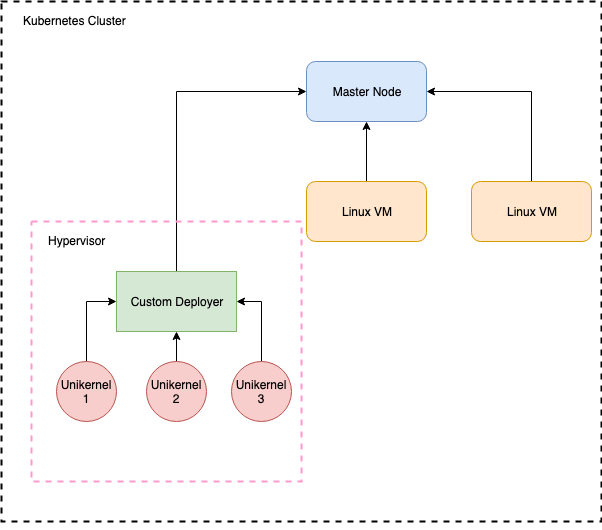
\includegraphics[width=0.8\textwidth]{figures/arch3.png}
  \caption{A kubernetes cluster with a only hypervisor enabled node for unikernel deployment} \label{fig:hypervisor}
\end{figure}
